\uuid{Dimq}
\exo7id{5062}
\titre{exo7 5062}
\auteur{quercia}
\organisation{exo7}
\datecreate{2010-03-17}
\isIndication{false}
\isCorrection{true}
\chapitre{Surfaces}
\sousChapitre{Surfaces paramétrées}
\module{Géométrie}
\niveau{L2}
\difficulte{}

\contenu{
\texte{
Soit $(\Gamma)$ : $\begin{cases} x(t) = a\cos(t)/\ch(mt)\cr
                          y(t) = a\sin(t)/\ch(mt)\cr
                          z(t) = a\tanh(mt).\cr\end{cases}$
}
\begin{enumerate}
    \item \question{Montrer que $(\Gamma)$ est tracée sur une surface $(\Sigma)$ simple. Montrer que $(\Sigma)$
    est de révolution autour de $Oz$ et donner son équation.}
\reponse{$x^2+y^2+z^2=a^2$.}
    \item \question{Montrer que $(\Gamma)$ coupe les méridiennes de $(\Sigma)$ suivant un angle constant (loxodromie).}
\reponse{On paramètre $(\Sigma)$ par :
             $\begin{cases} x = a\cos u/\ch v\cr y = a\sin u/\sh v\cr z = a\tanh v.\cr\end{cases}$\par
        La tangente à la méridienne passant par $M(u,v)$ est dirigée par $\frac{\partial {\vec M}}{\partial v}$ et la tangente à $(\Gamma)$ passant par $M(t,mt)$ est dirigée par $\frac{\partial  {\vec M}}{\partial u} + m\frac{\partial {\vec M}}{\partial v}$. Après calculs, le cosinus de ces deux vecteurs vaut $\frac m{\sqrt{m^2+1}}$ donc est constant.}
    \item \question{Réciproquement, déterminer toutes les loxodromies de $(\Sigma)$.}
\reponse{Une courbe tracée sur $(\Sigma)$ est définie par la donnée de $u$ et $v$ en fonction d'un paramètre $t$. Le cosinus de l'angle entre cette courbe et une méridienne de $(\Sigma)$ vaut $\frac{u'}{\sqrt{u'^2+v'^2}}$, donc est constant si et seulement si le rapport \frac{v'}{u'}$ est constant. En notant $m$ cette constante et en prenant $u(t)=t$, on trouve les courbes déduites de $(\Gamma)$ par rotation autour de $Oz$.}
    \item \question{Dessiner la projection de $(\Gamma)$ sur $xOy$.}
\reponse{$$\centerline{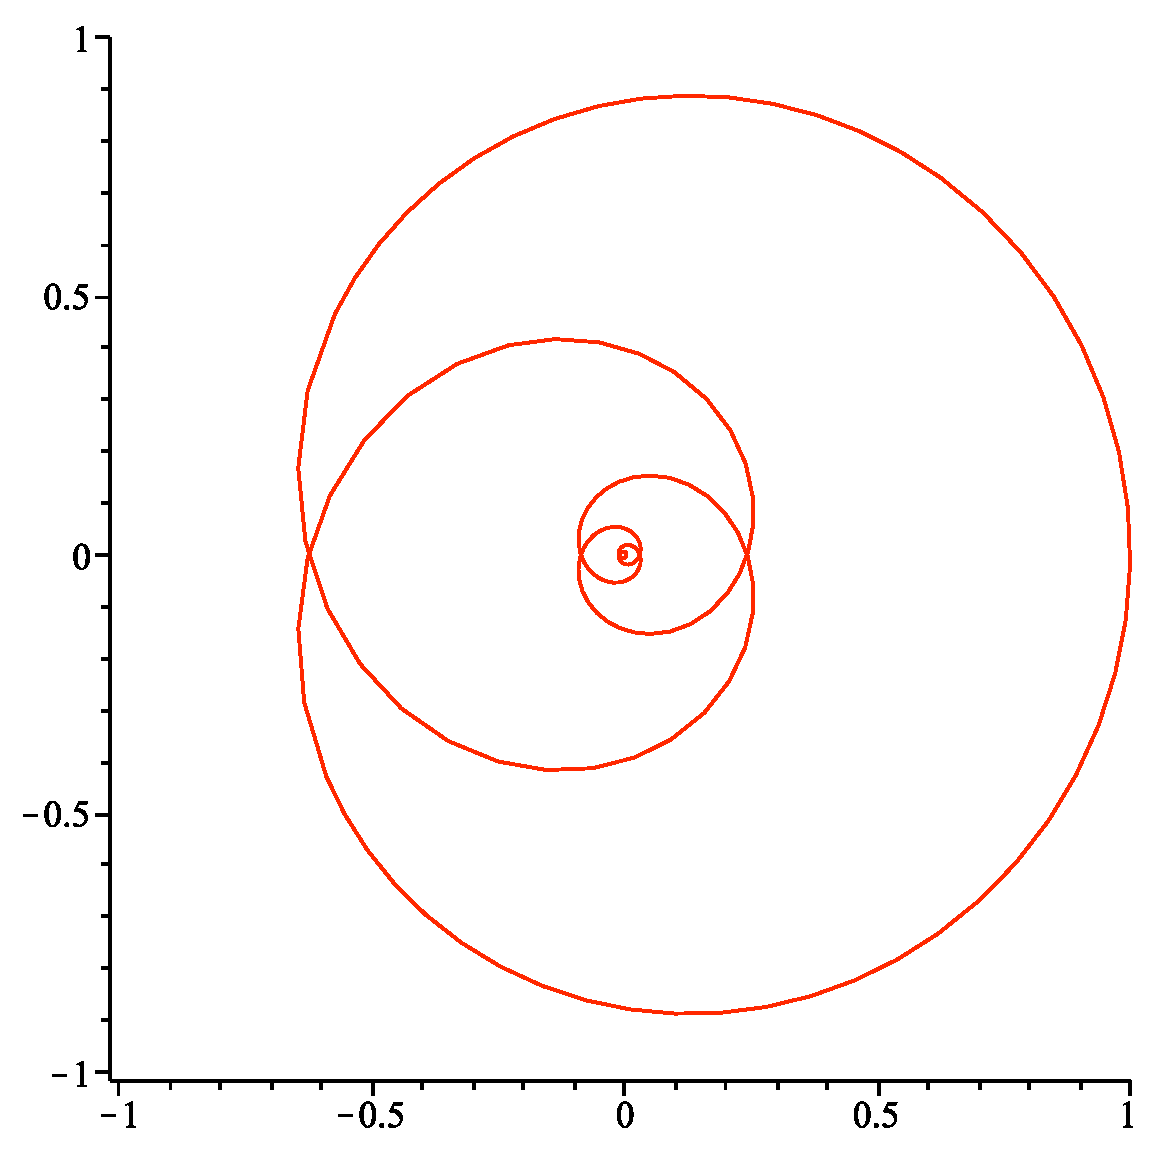
\includegraphics[height=4cm]{../images/pdf/Dimq-1.pdf}}$$
%     \mapleplot{plot([1/cosh(t/3),t,t=-20..20],view=[-1..1,-1..1],coords=polar,axes=frame);}
%     \hbox{\indent équation polaire $\rho = \frac{a}{\ch m\theta}$.}}
\end{enumerate}
}
